\chapter{End-use case studies}
\section{Precise forestry}
\subsection{Terrestrial laser scanning}

\begin{figure}[H]
	\centering
	\includegraphics[width=0.5\textwidth]{precise_forestry/Zdjęcie WhatsApp 2025-02-01 o 18.10.13_85222b6b.jpg}
	\caption{Hardware: Mandeye Mission Recorder + Livox AVIA + tripod.}
	\label{fig:pf1}
\end{figure}

\begin{figure}[H]
	\centering
	\includegraphics[width=0.5\textwidth]{precise_forestry/Zdjęcie WhatsApp 2025-02-01 o 18.10.13_c8c96bab.jpg}
	\caption{Hardware: Mandeye Mission Recorder + Livox AVIA + tripod.}
	\label{fig:pf2}
\end{figure}

\begin{figure}[H]
	\centering
	\includegraphics[width=0.5\textwidth]{precise_forestry/Zdjęcie WhatsApp 2025-02-01 o 18.10.13_ff03d501.jpg}
	\caption{Hardware: Mandeye Mission Recorder + Livox AVIA + tripod.}
	\label{fig:pf3}
\end{figure}


\begin{figure}[H]
	\centering
	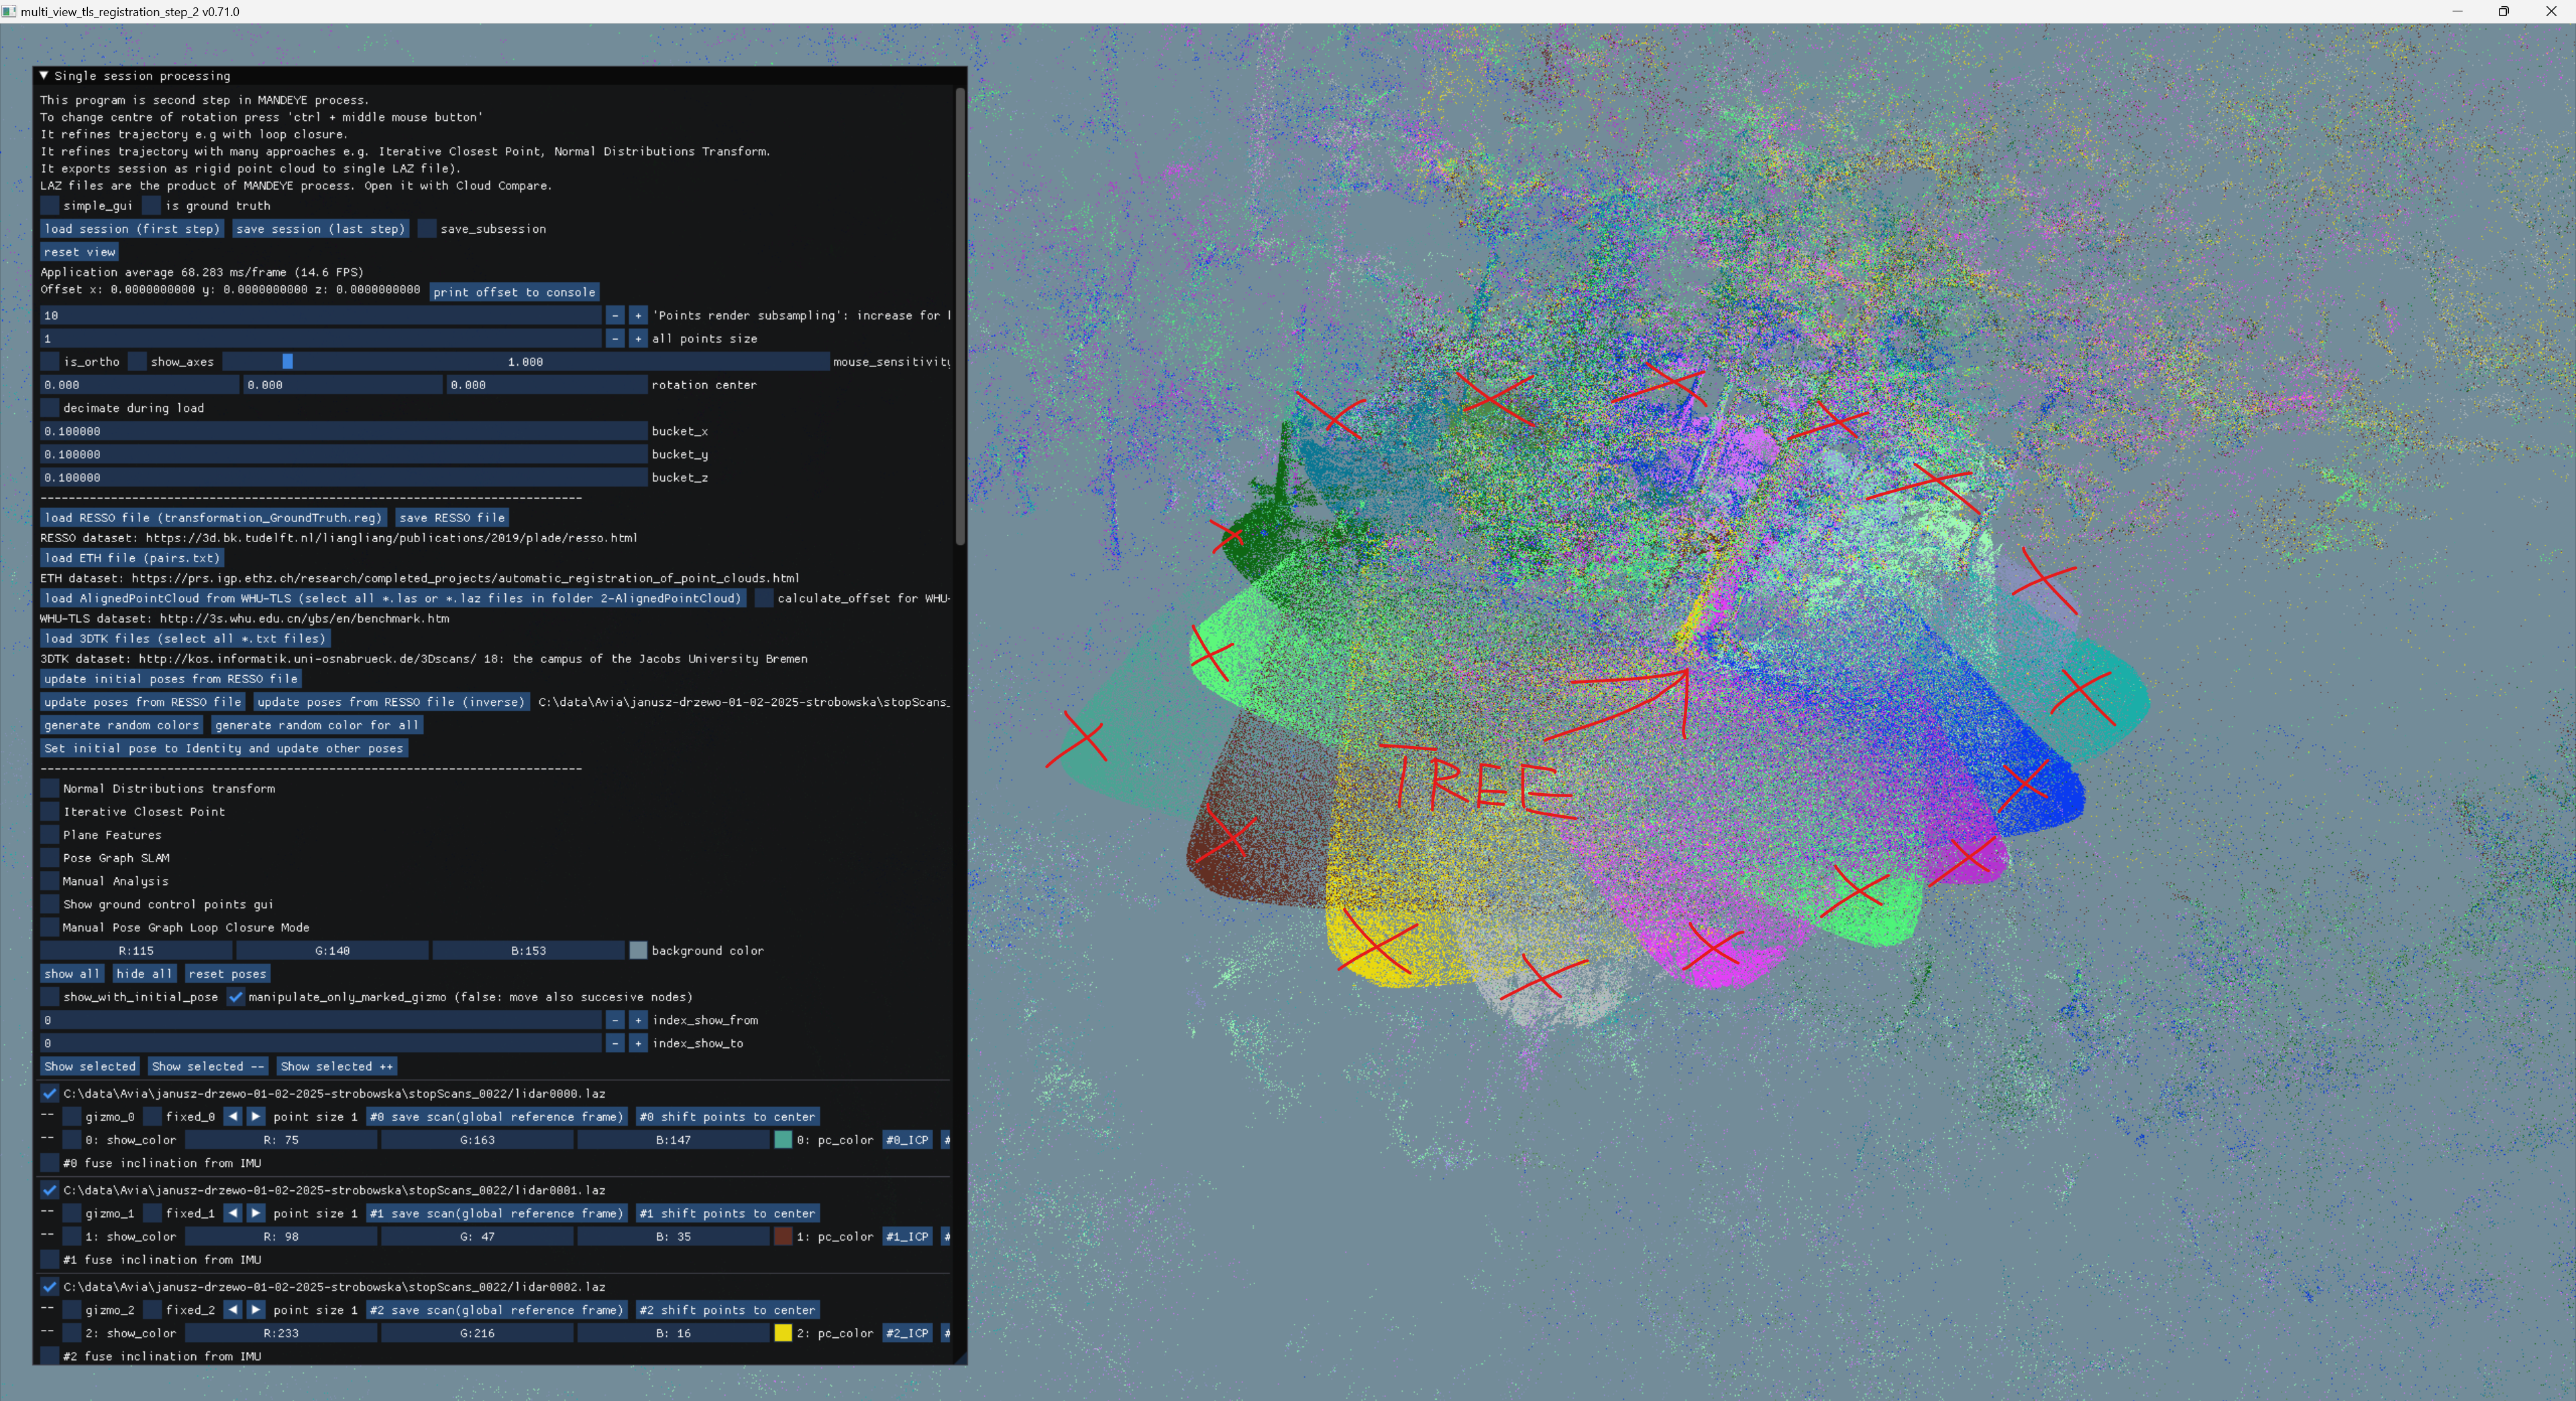
\includegraphics[width=1.0\textwidth]{precise_forestry/Zrzut ekranu 2025-02-01 184408.png}
	\caption{Data collection strategy: multiple STOP SCANS around the tree.}
	\label{fig:pf22}
\end{figure}

\begin{figure}[H]
	\centering
	\includegraphics[width=1.0\textwidth]{precise_forestry/tree.png}
	\caption{Objective: registered data.}
	\label{fig:pf4}
\end{figure}

\begin{figure}[H]
	\centering
	\includegraphics[width=1.0\textwidth]{precise_forestry/tree2.png}
	\caption{Objective: registered data.}
	\label{fig:pf5}
\end{figure}

\begin{figure}[H]
	\centering
	\includegraphics[width=1.0\textwidth]{precise_forestry/Zrzut ekranu 2025-02-01 165606.png}
	\caption{Step1: open 'multi\_view\_tls\_registration\_step\_2' program version >= 0.72 and umark 'simple\_gui'.}
	\label{fig:pf6}
\end{figure}

\begin{figure}[H]
	\centering
	\includegraphics[width=1.0\textwidth]{precise_forestry/Zrzut ekranu 2025-02-01 165647.png}
	\caption{Step2: Load data using button 'load AlignedPointCloud from WHI-TLS'.}
	\label{fig:pf7}
\end{figure}

\begin{figure}[H]
	\centering
	\includegraphics[width=1.0\textwidth]{precise_forestry/Zrzut ekranu 2025-02-01 165800.png}
	\caption{Step3: Mark all *.laz files collected by MANDEYE MISSION RECORDER.}
	\label{fig:pf8}
\end{figure}

\begin{figure}[H]
	\centering
	\includegraphics[width=1.0\textwidth]{precise_forestry/Zrzut ekranu 2025-02-01 165834.png}
	\caption{Step4: Read info.}
	\label{fig:pf9}
\end{figure}

\begin{figure}[H]
	\centering
	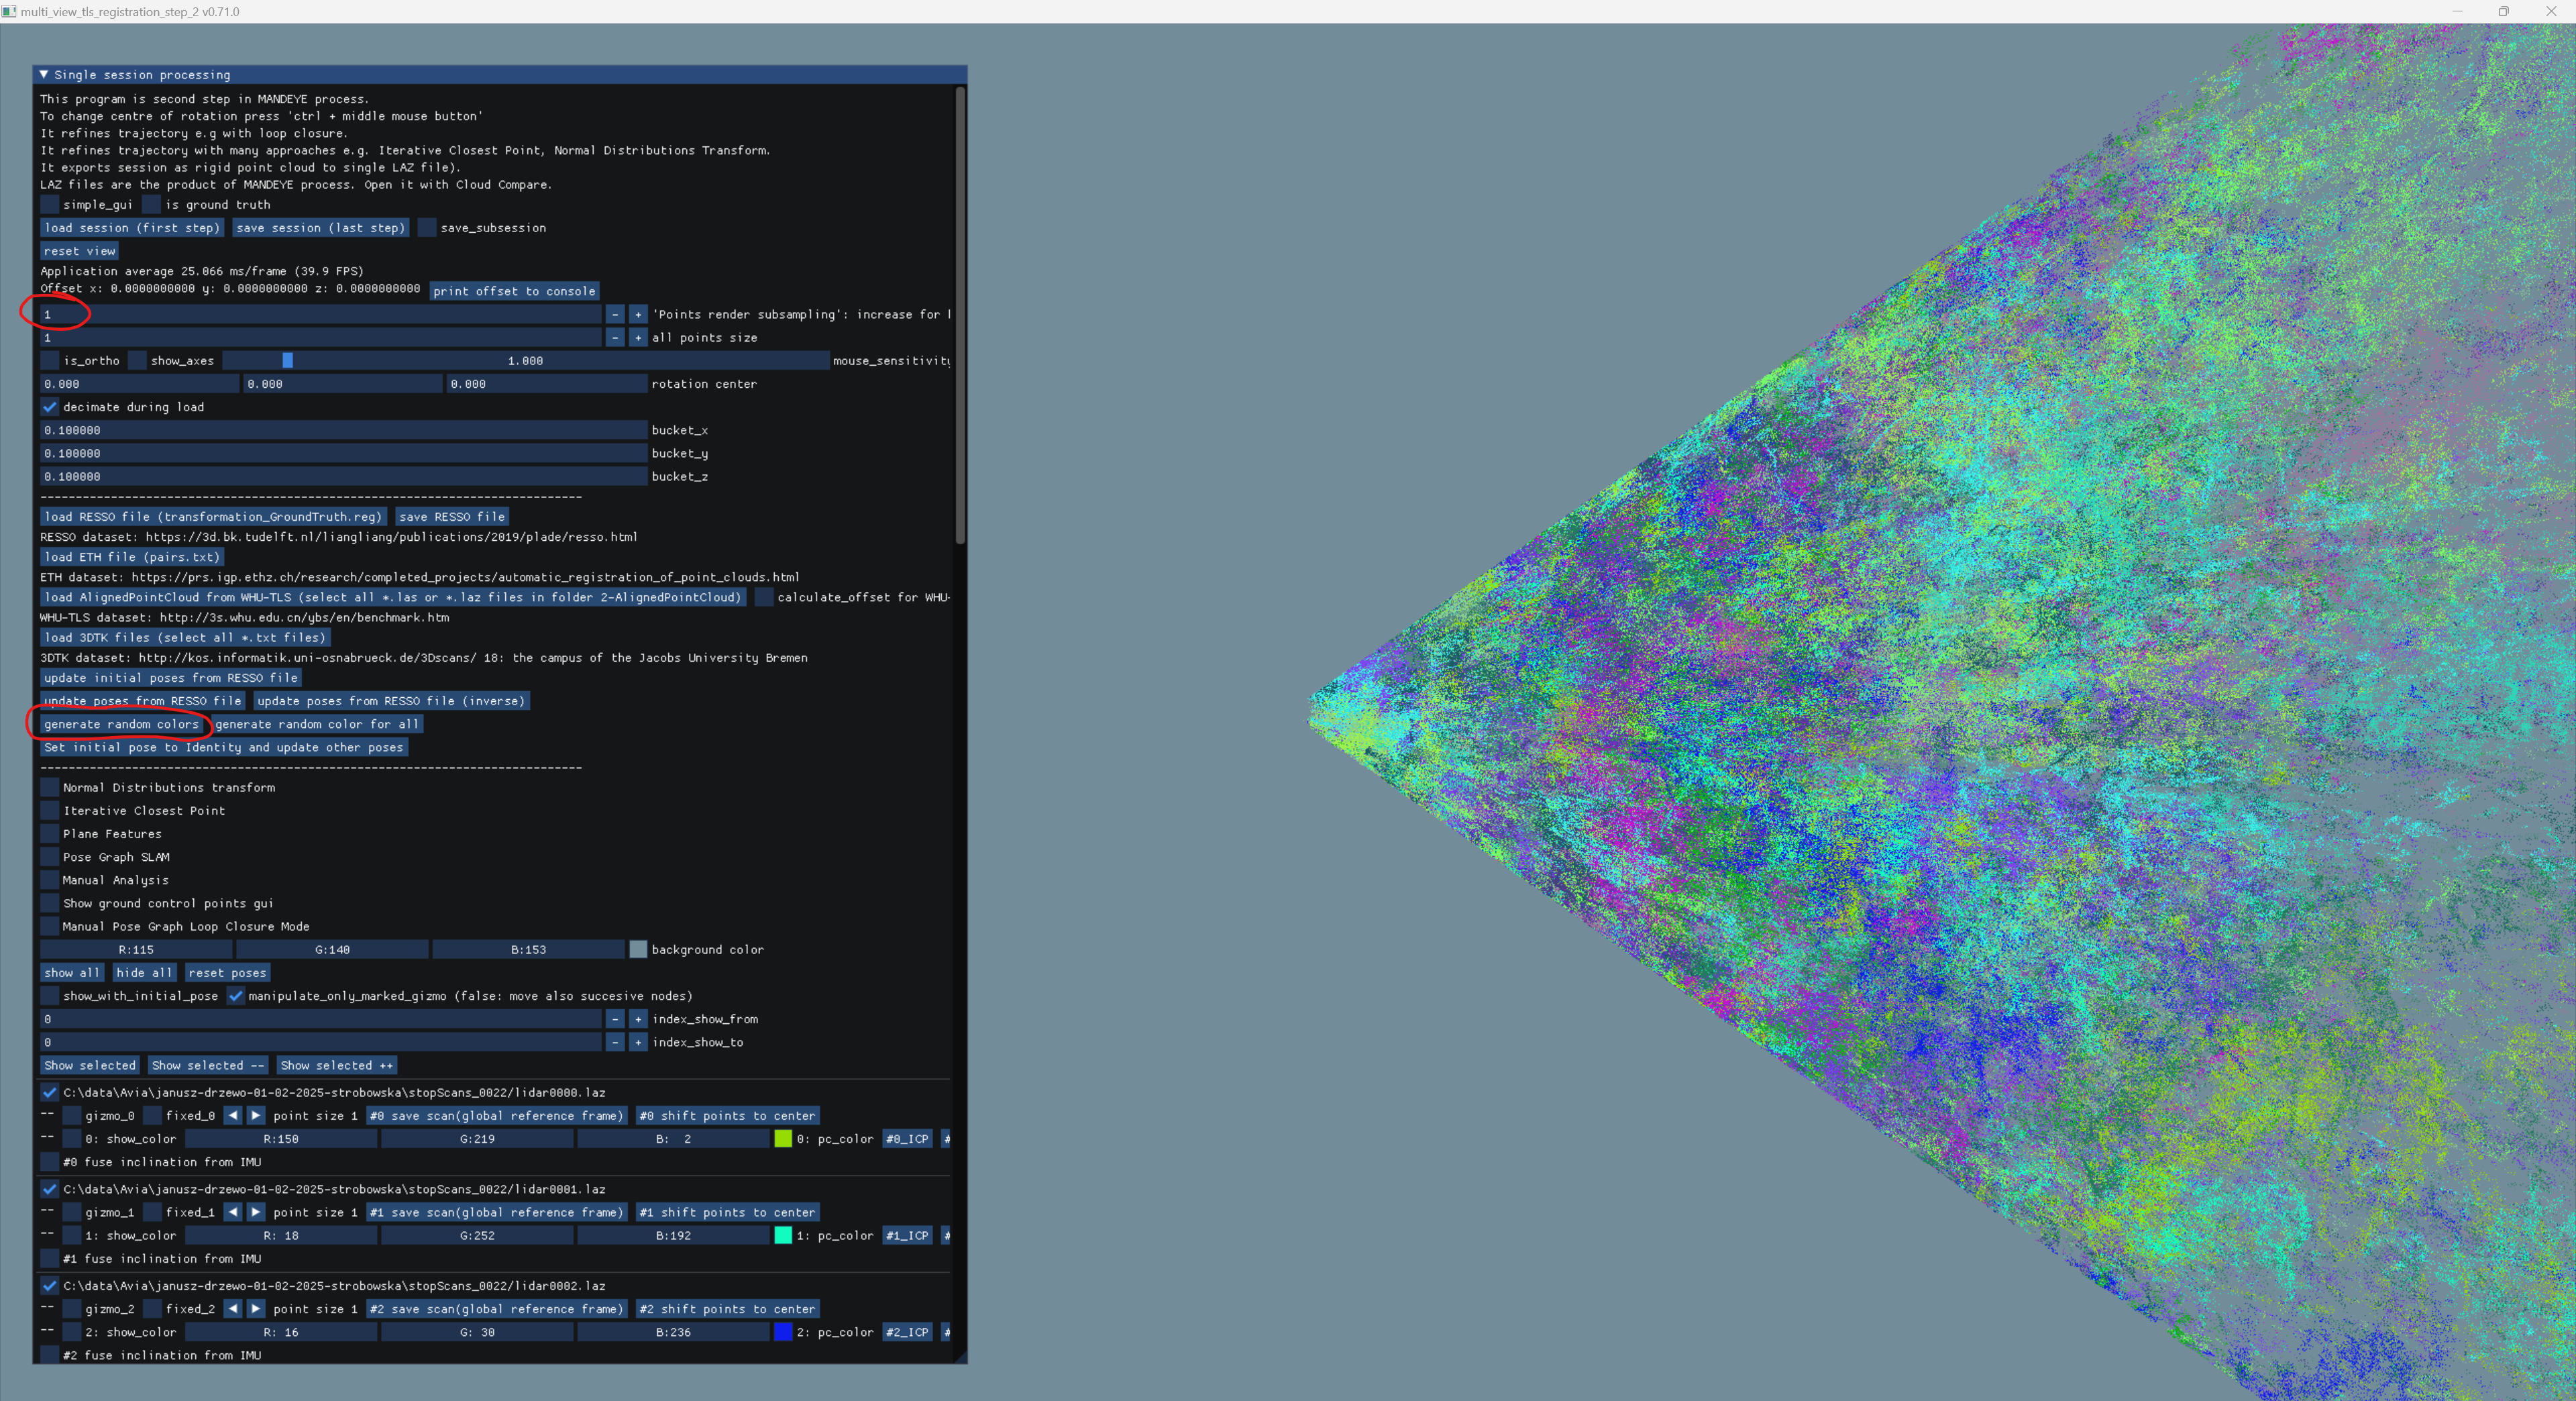
\includegraphics[width=1.0\textwidth]{precise_forestry/Zrzut ekranu 2025-02-01 165912.png}
	\caption{Step5: Change 'Points render subsampling' and press 'generate random colors'.}
	\label{fig:pf10}
\end{figure}

\begin{figure}[H]
	\centering
	\includegraphics[width=1.0\textwidth]{precise_forestry/Zrzut ekranu 2025-02-01 170004.png}
	\caption{Step6: Press 'hide all', check first and second point cloud, check 'gizmo' for second point cloud.}
	\label{fig:pf11}
\end{figure}

\begin{figure}[H]
	\centering
	\includegraphics[width=1.0\textwidth]{precise_forestry/Zrzut ekranu 2025-02-01 170055.png}
	\caption{Step7: Move second point cloud by gizmo and press '1_ICP' to align second point cloud to previous one.}
	\label{fig:pf12}
\end{figure}

\begin{figure}[H]
	\centering
	\includegraphics[width=1.0\textwidth]{precise_forestry/Zrzut ekranu 2025-02-01 170143.png}
	\caption{Step8: Uncheck 'gizmo' then press '1_ICP'!.}
	\label{fig:pf13}
\end{figure}

\begin{figure}[H]
	\centering
	\includegraphics[width=1.0\textwidth]{precise_forestry/Zrzut ekranu 2025-02-01 180813.png}
	\caption{Step9: Repeat this procedure for all consecutive pairs of scans.}
	\label{fig:pf14}
\end{figure}

\begin{figure}[H]
	\centering
	\includegraphics[width=1.0\textwidth]{precise_forestry/Zrzut ekranu 2025-02-01 180851.png}
	\caption{Step10: Check 'Normal Distributions Transform' and press 'ndt\_optimization'.}
	\label{fig:pf15}
\end{figure}



\begin{figure}[H]
	\centering
	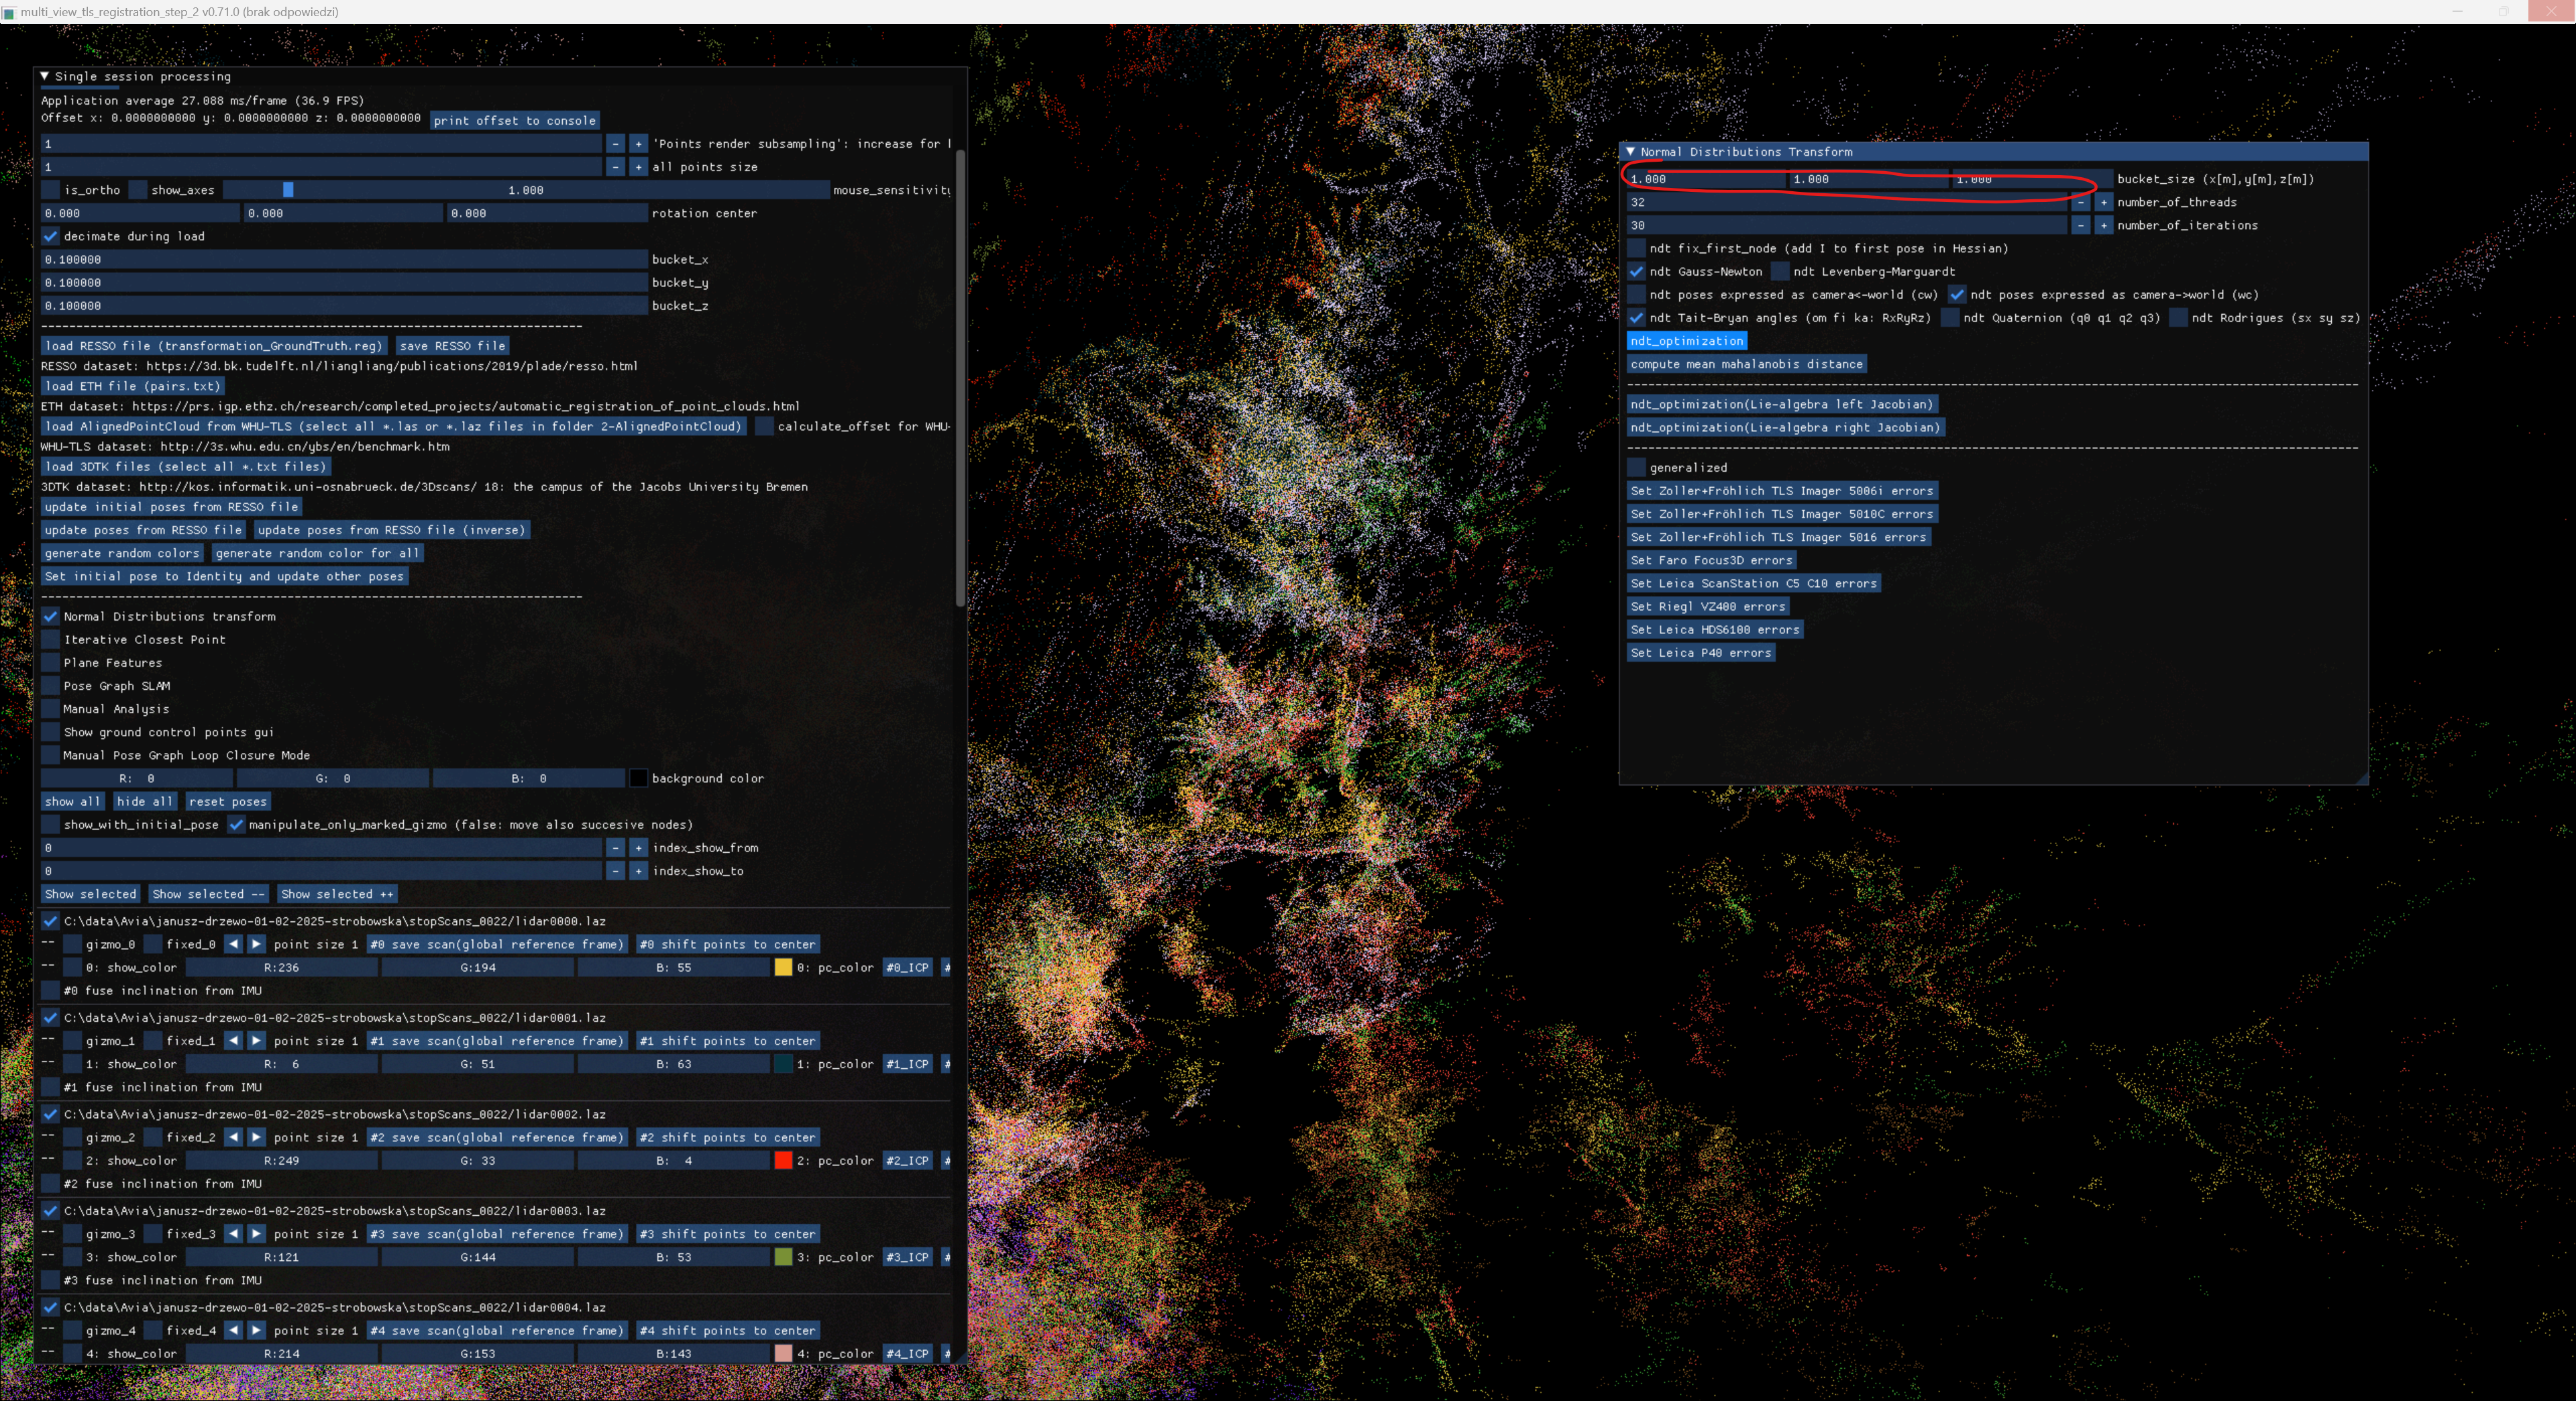
\includegraphics[width=1.0\textwidth]{precise_forestry/Zrzut ekranu 2025-02-01 182915.png}
	\caption{Step12: If You are not satisfied with the result change bucket size to 1,1,1 and press 'ndt\_optimization'.}
	\label{fig:pf17}
\end{figure}

\begin{figure}[H]
	\centering
	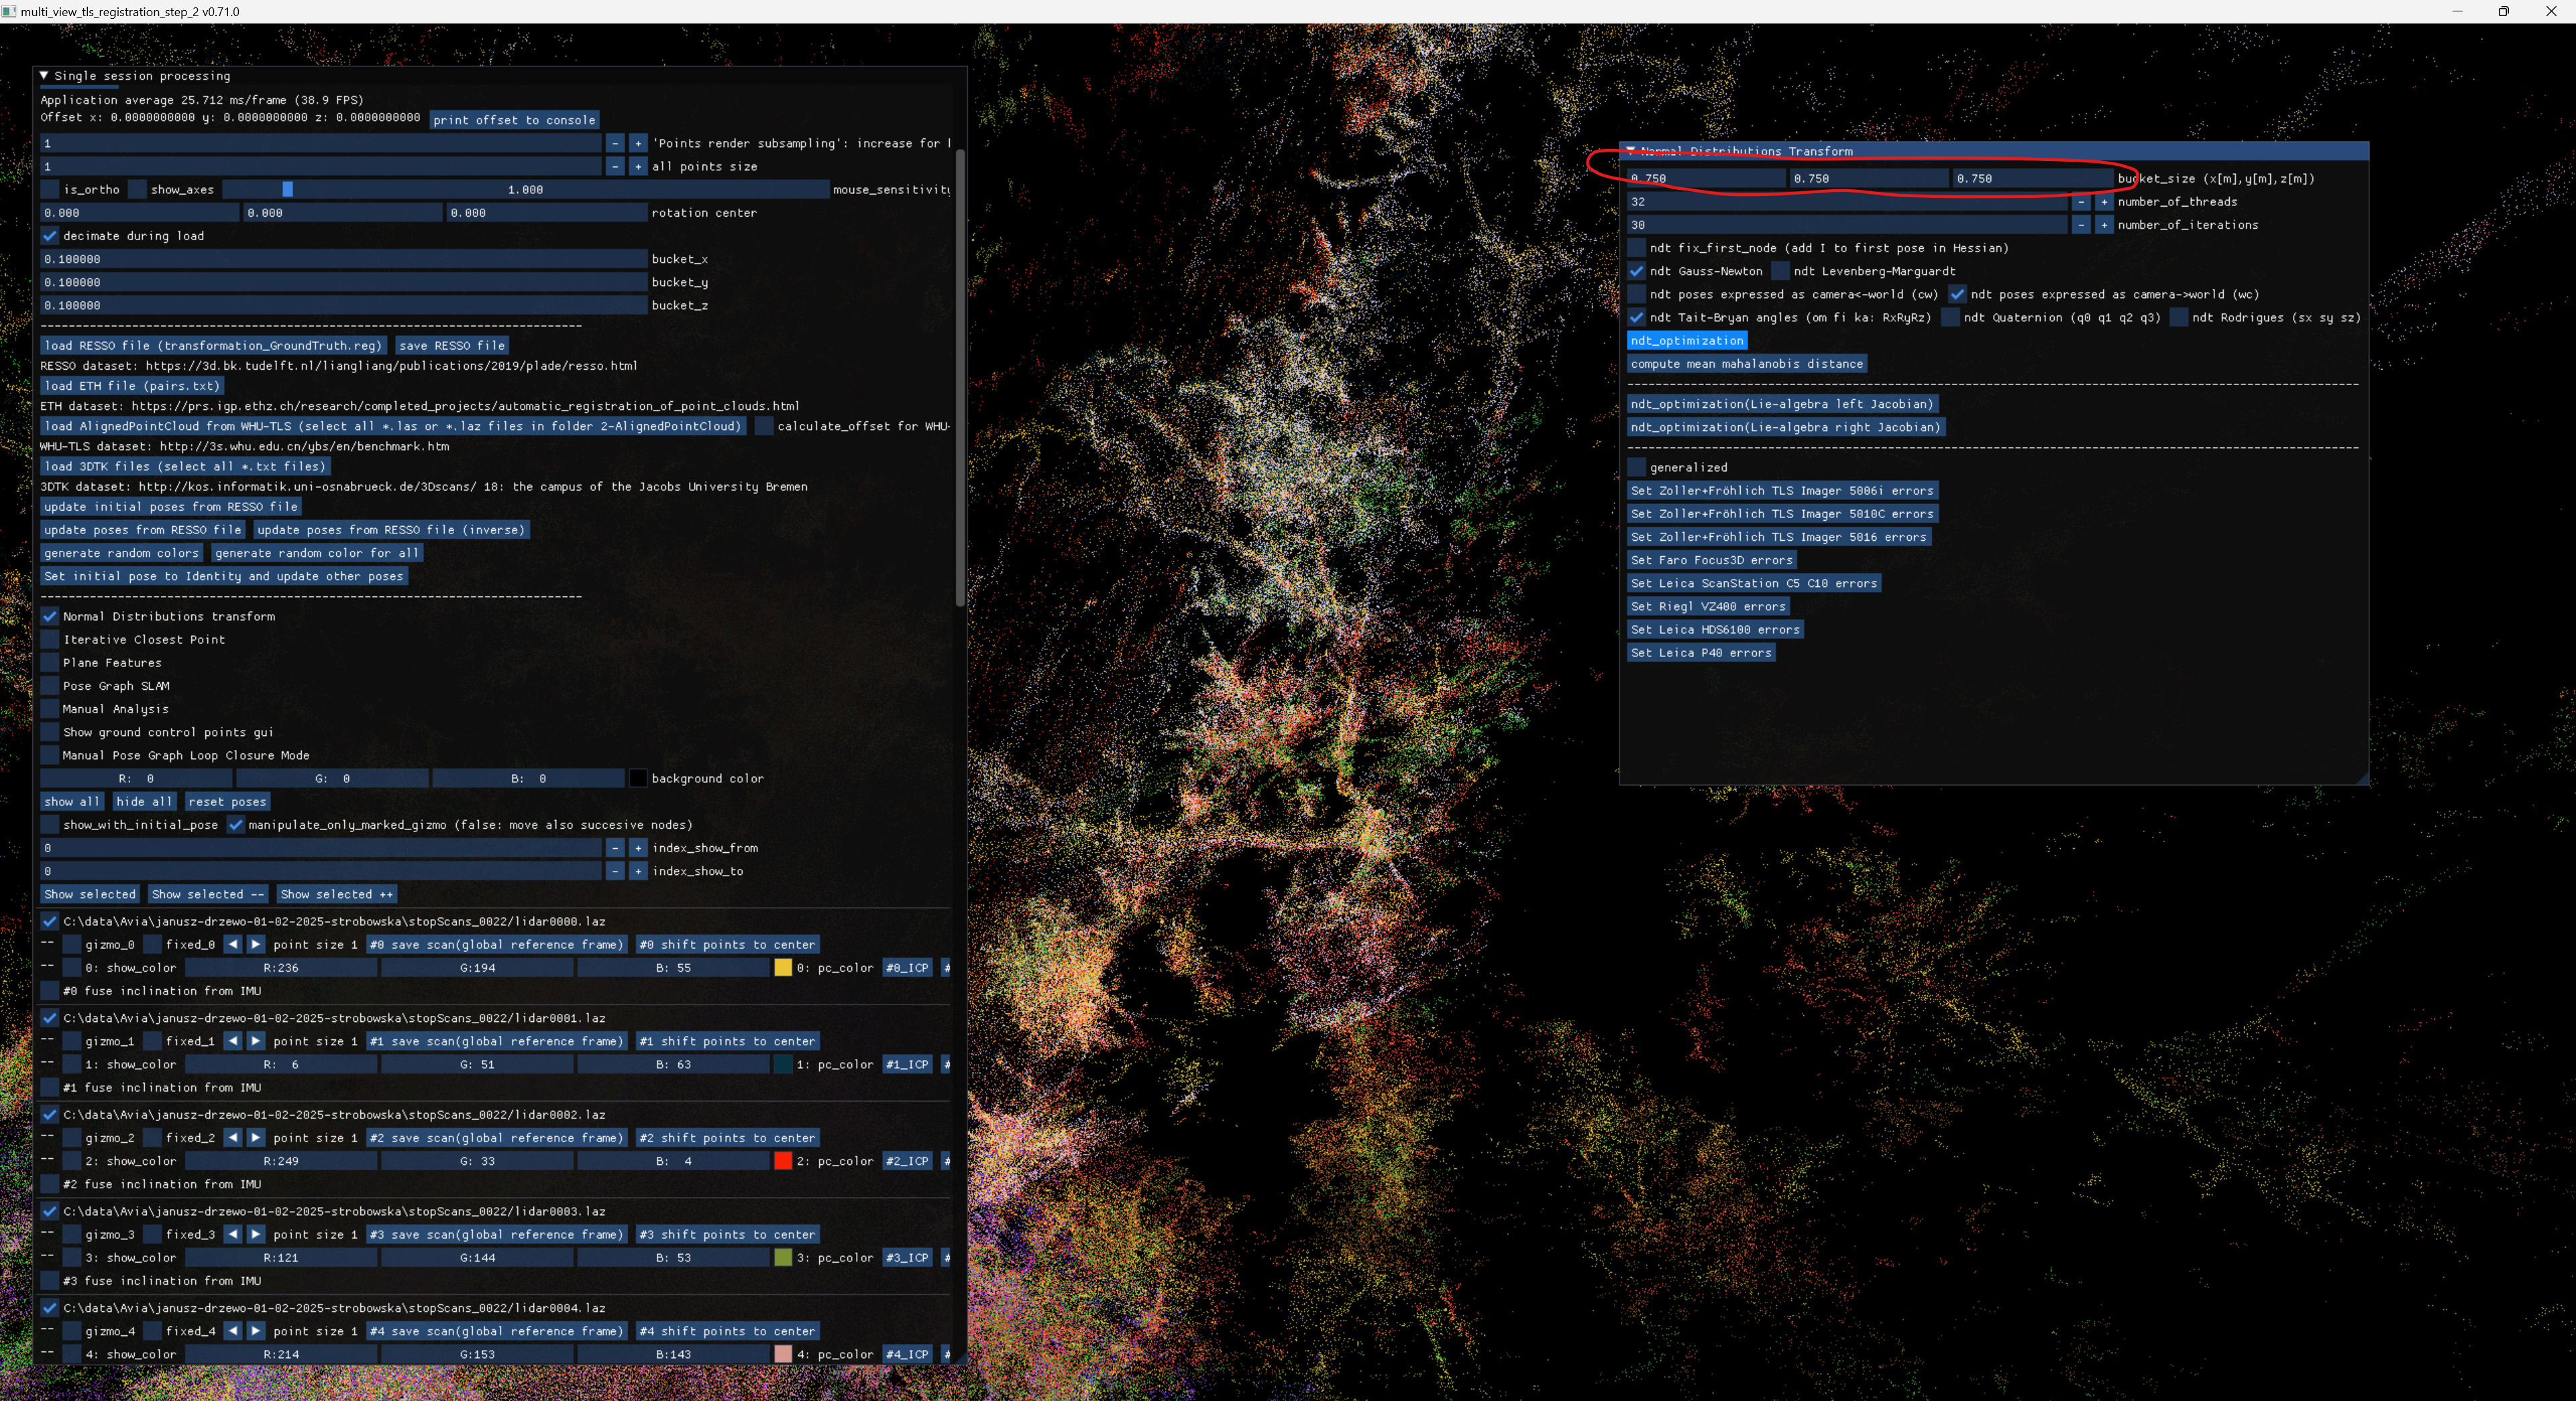
\includegraphics[width=1.0\textwidth]{precise_forestry/Zrzut ekranu 2025-02-01 183150.png}
	\caption{Step13: If You are not satisfied with the result change bucket size to 0.75,0.75,0.75 and press 'ndt\_optimization'.}
	\label{fig:pf18}
\end{figure}

\begin{figure}[H]
	\centering
	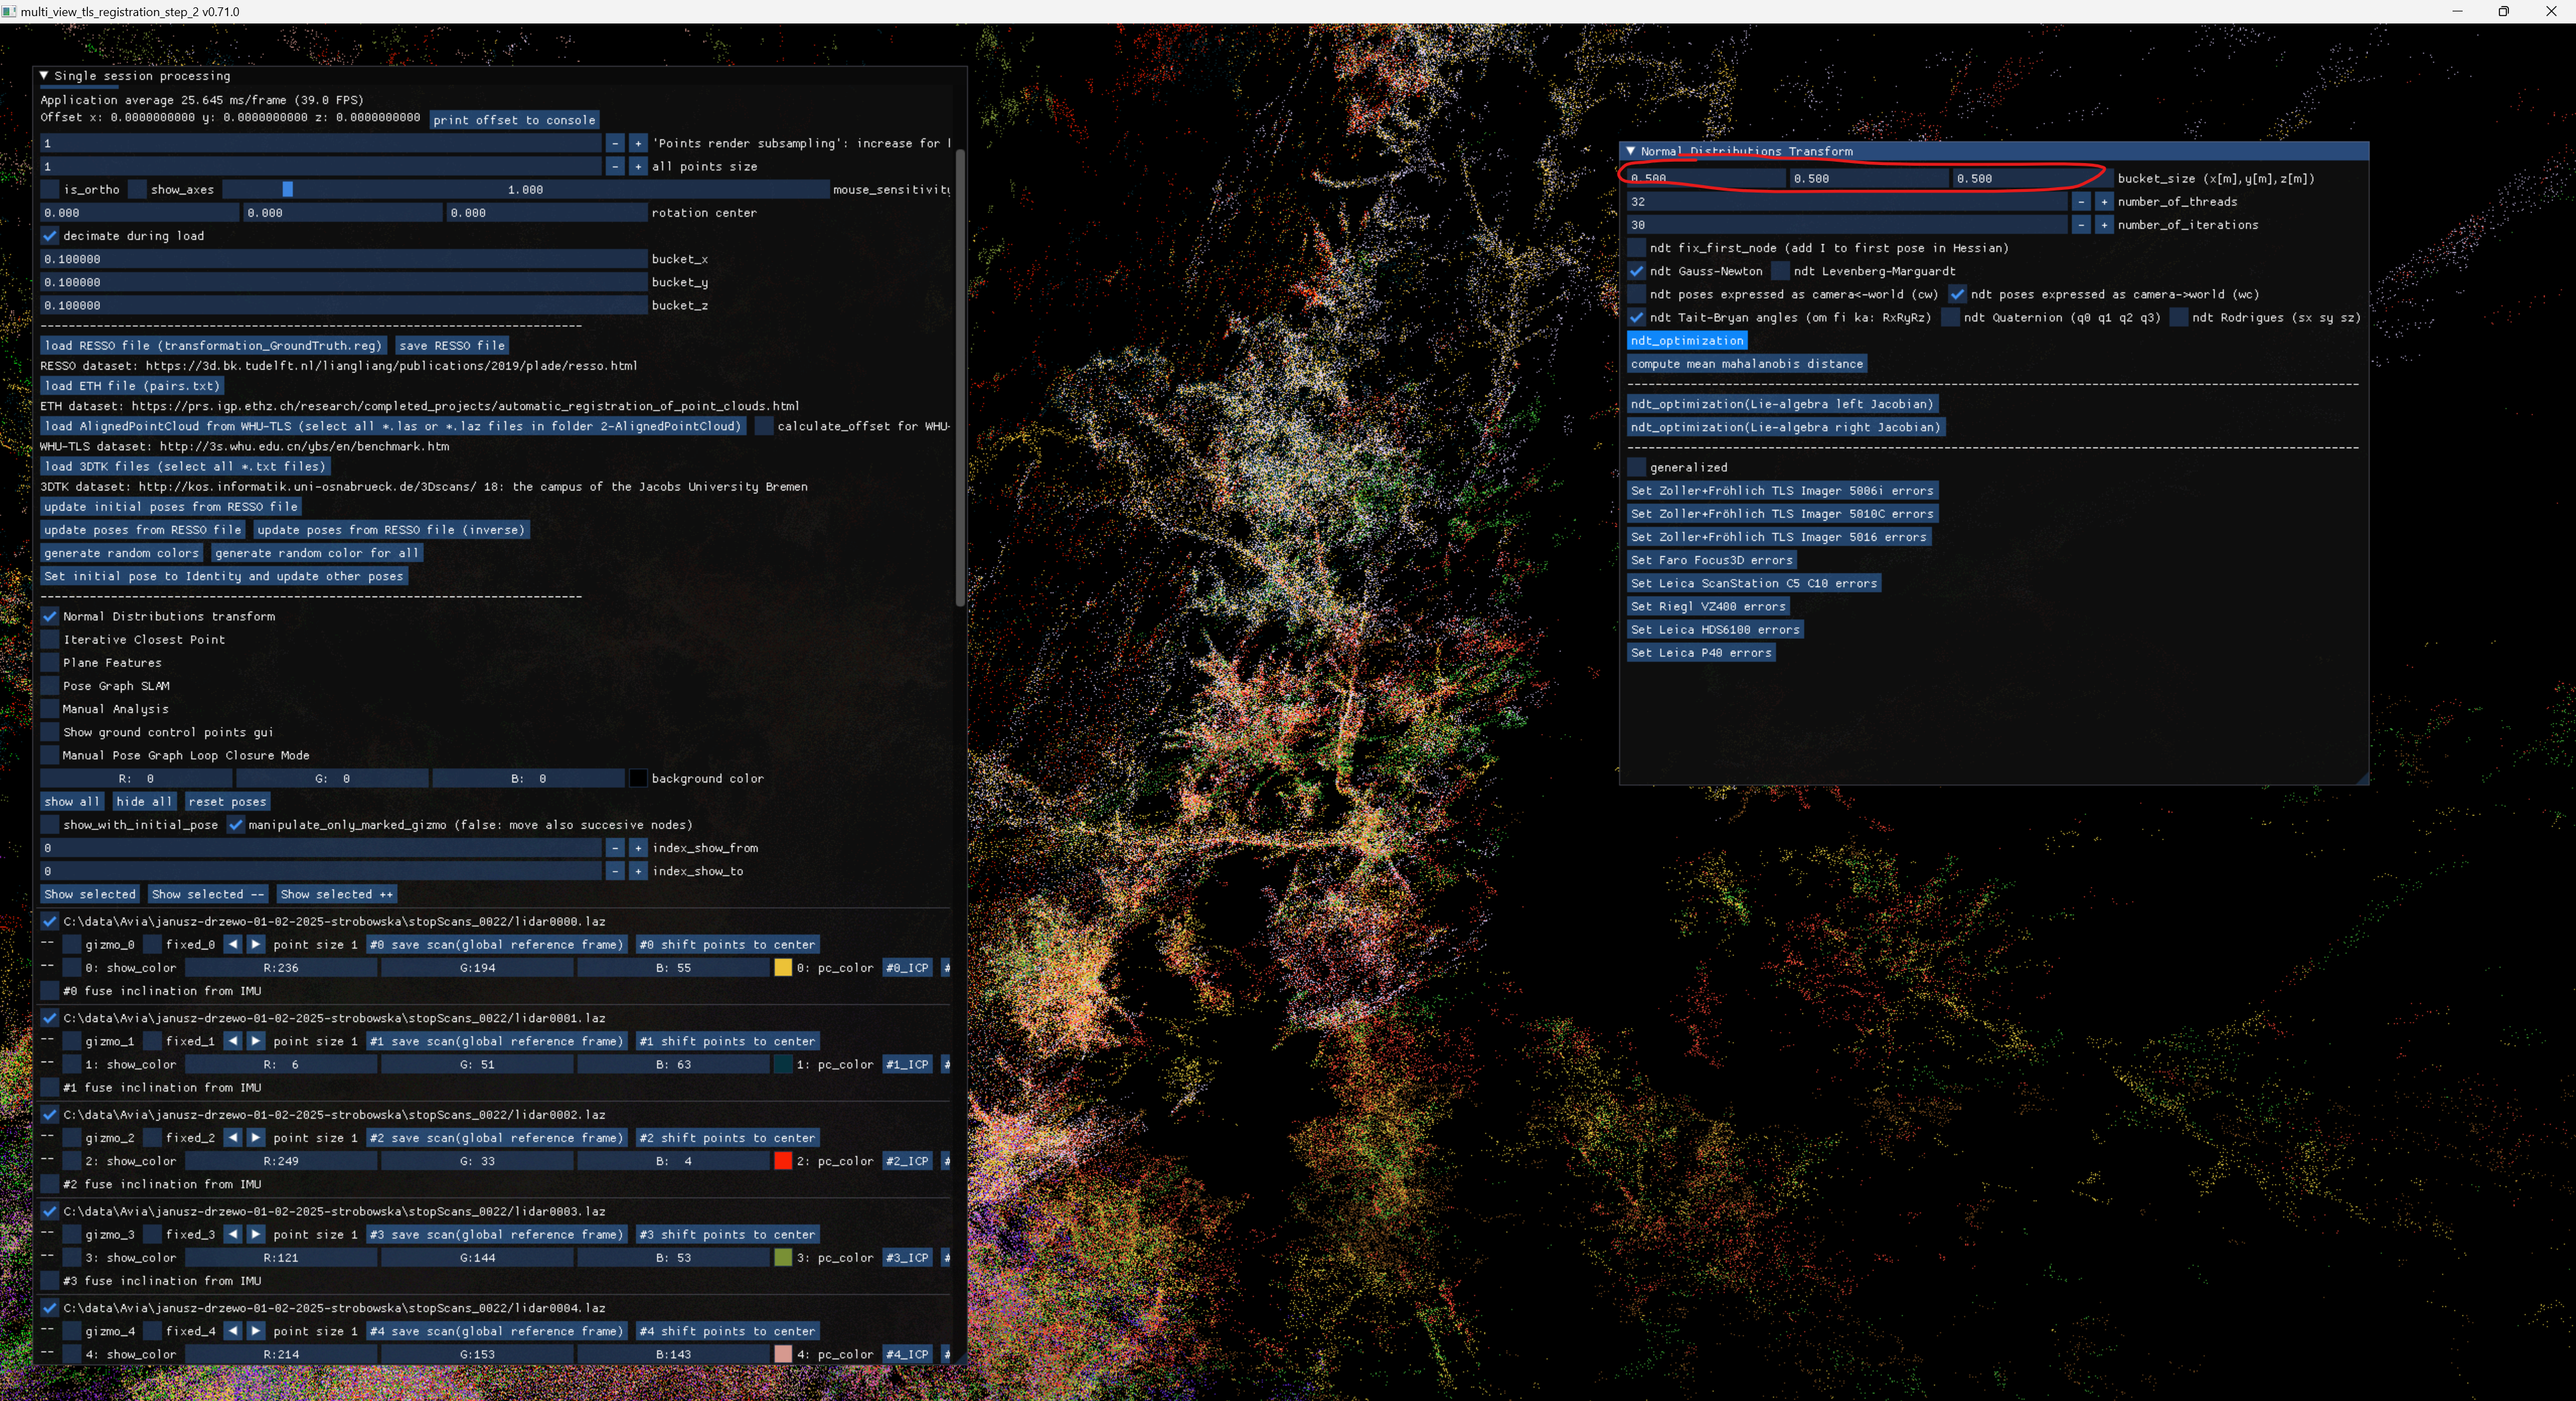
\includegraphics[width=1.0\textwidth]{precise_forestry/Zrzut ekranu 2025-02-01 183456.png}
	\caption{Step14: If You are not satisfied with the result change bucket size to 0.5,0.5,0.5 and press 'ndt\_optimization'.}
	\label{fig:pf19}
\end{figure}

\begin{figure}[H]
	\centering
	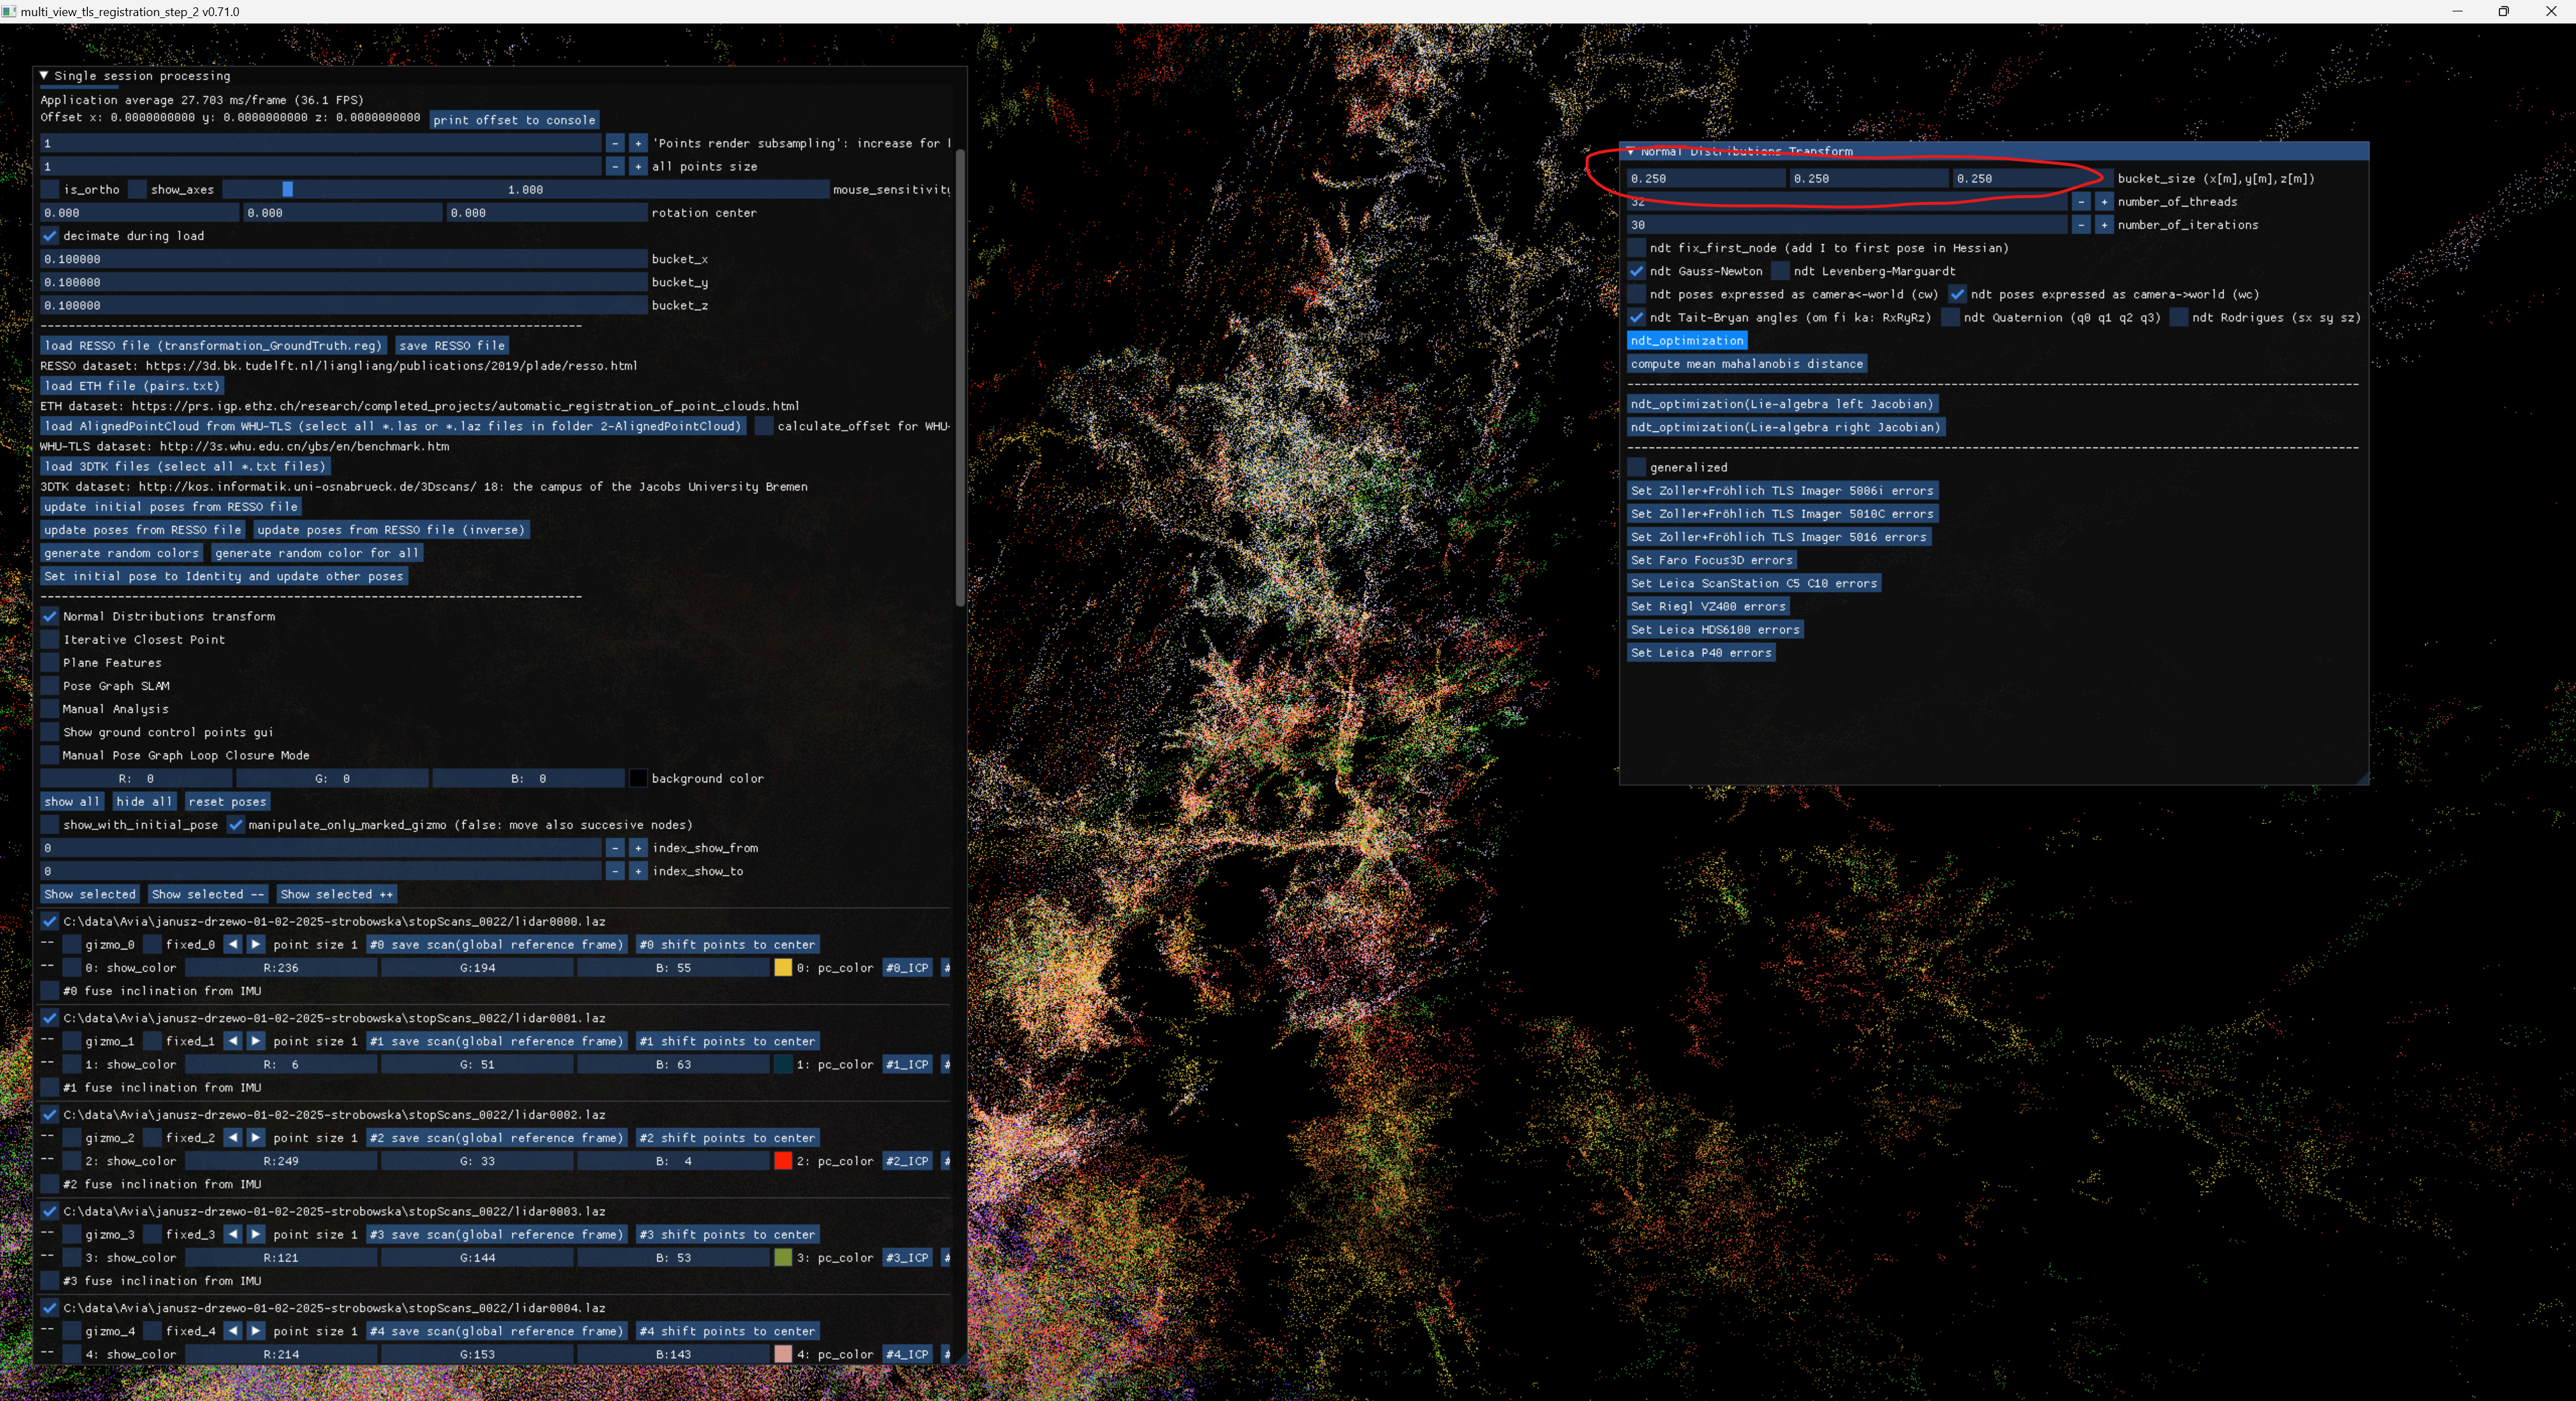
\includegraphics[width=1.0\textwidth]{precise_forestry/Zrzut ekranu 2025-02-01 183728.png}
	\caption{Step15: If You are not satisfied with the result change bucket size to 0.3,0.3,0.3 and press 'ndt\_optimization'.}
	\label{fig:pf20}
\end{figure}

\begin{figure}[H]
	\centering
	\includegraphics[width=1.0\textwidth]{precise_forestry/Zrzut ekranu 2025-02-01 181204-30iter.png}
	\caption{Step16: Save result as RESSO file.}
	\label{fig:pf16}
\end{figure}\\

\begin{figure}[H]
	\centering
	\includegraphics[width=1.0\textwidth]{precise_forestry/Zrzut ekranu 2025-02-01 184224.png}
	\caption{Step17: Load data in full resolution. Unmark 'simple\_gui', unmark 'decimation during load', load all data like in step2, update poses from RESSO file.  }
	\label{fig:pf21}
\end{figure}


\begin{figure}[H]
	\centering
	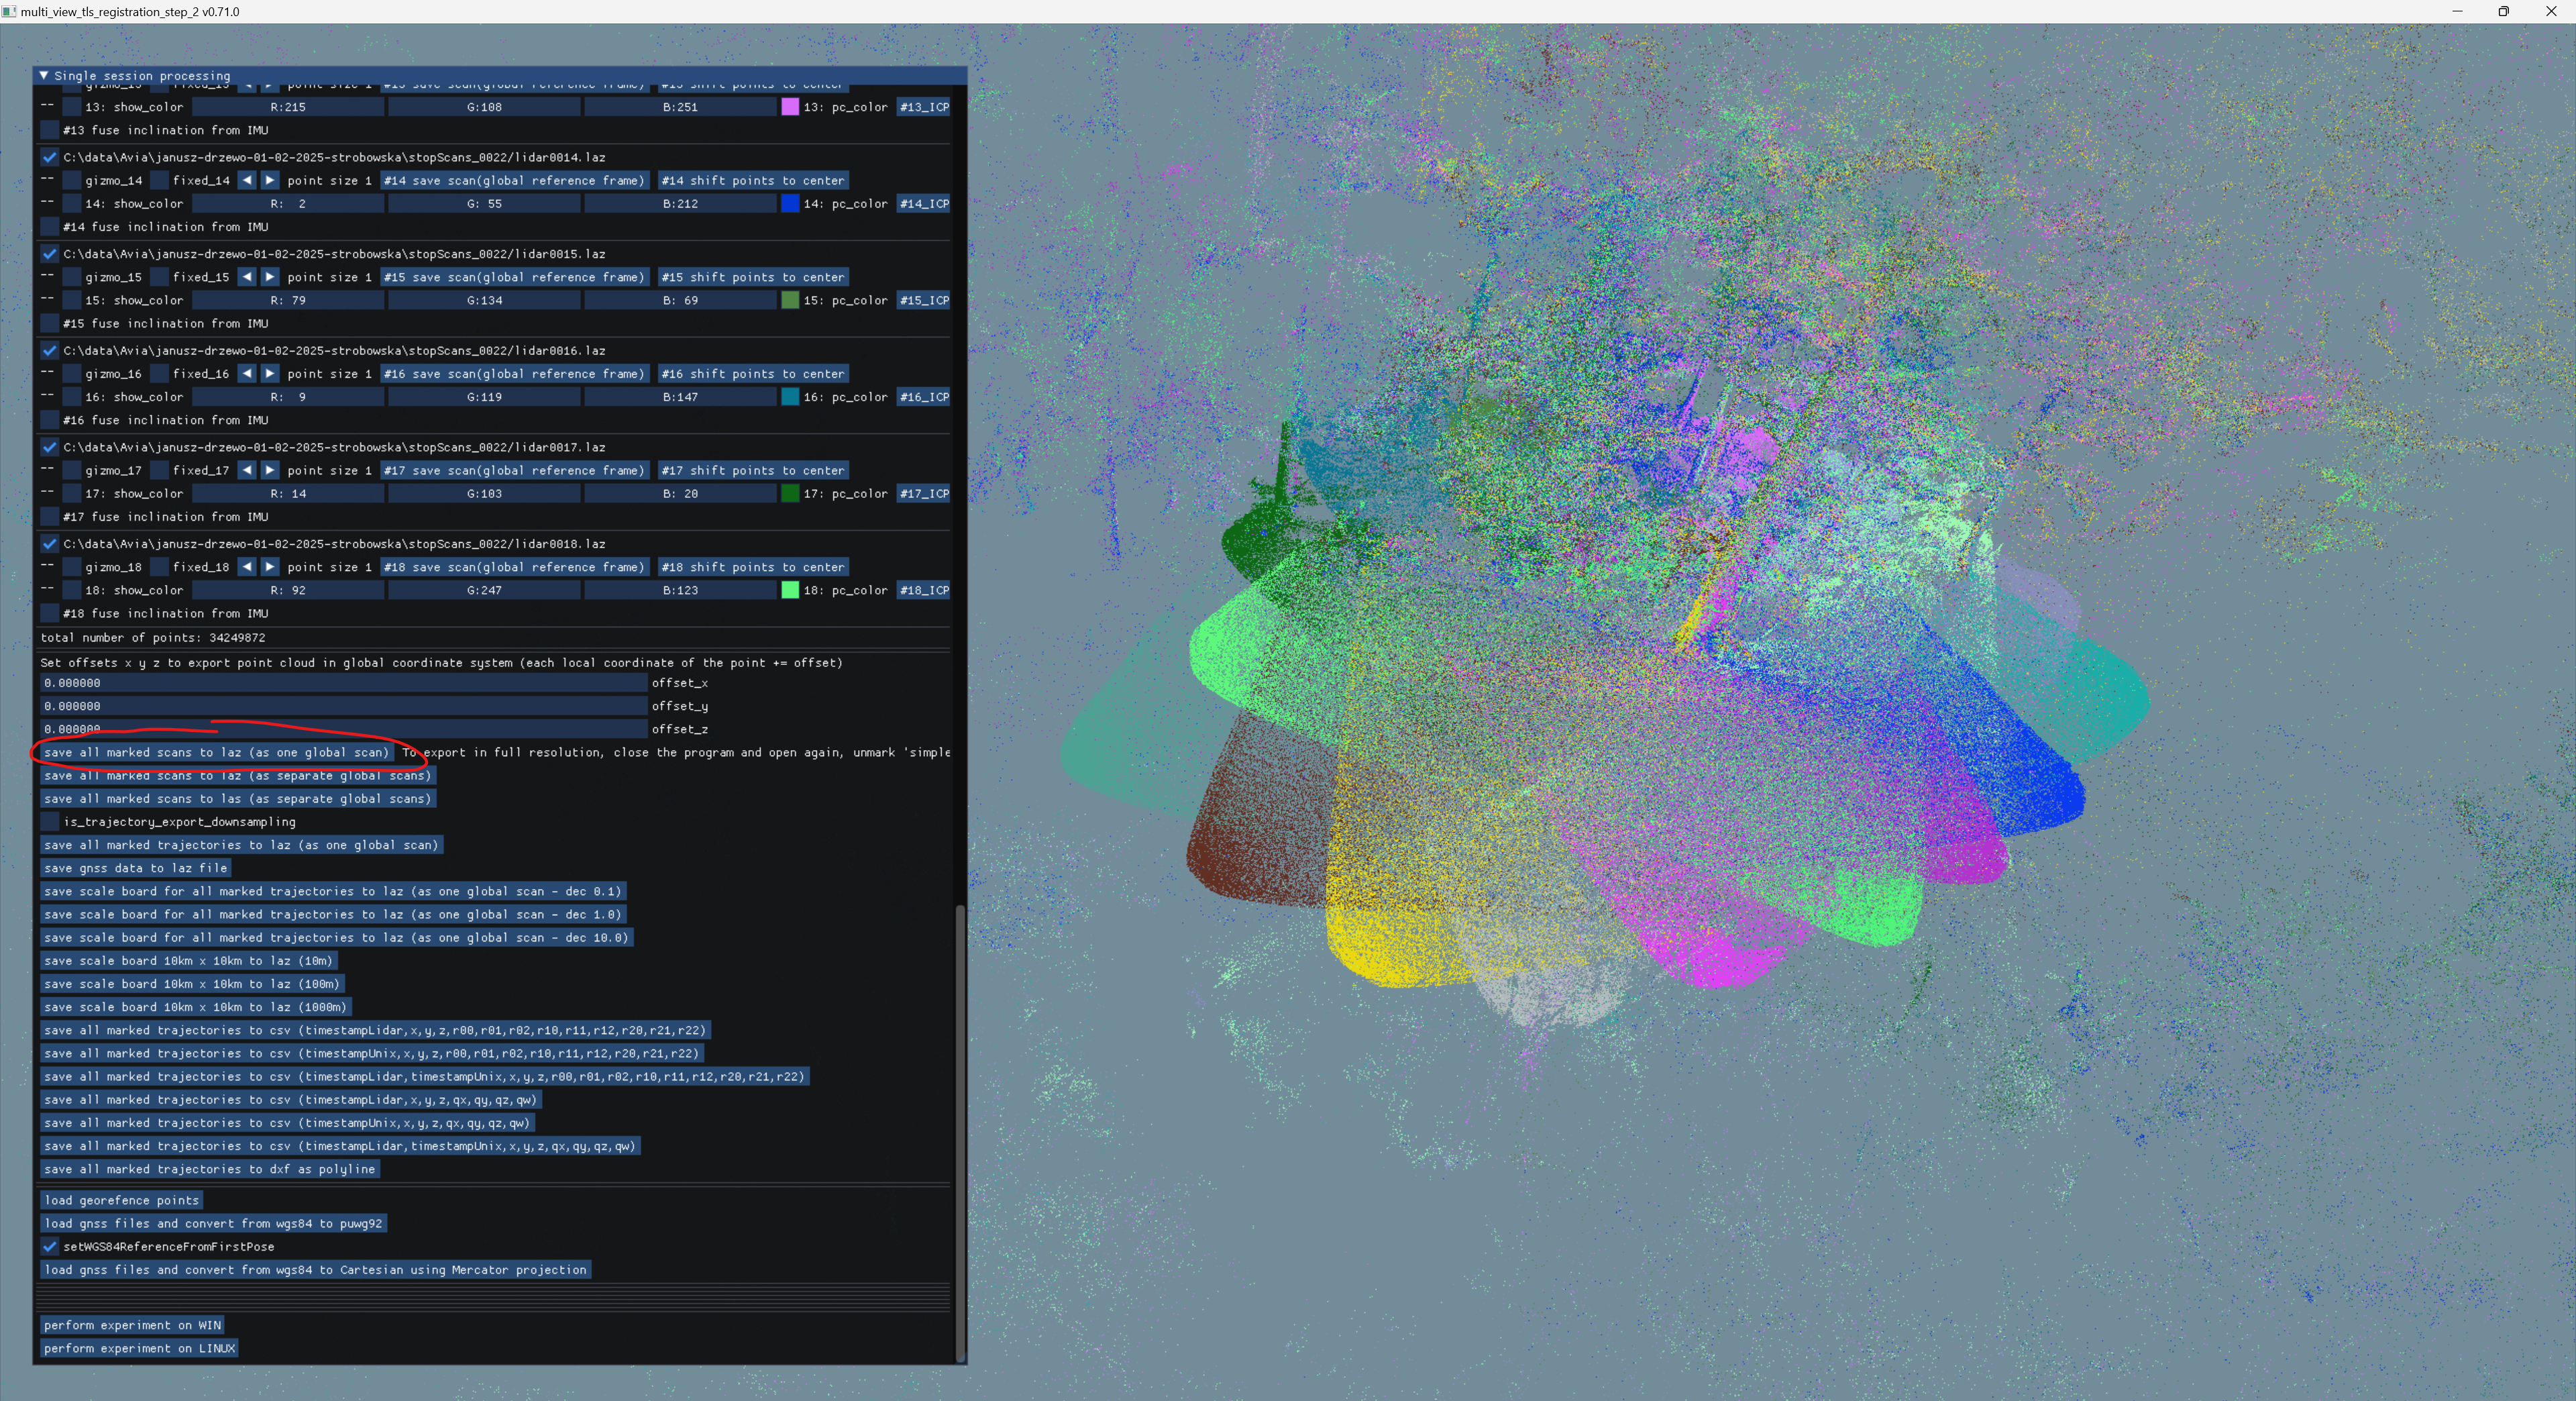
\includegraphics[width=1.0\textwidth]{precise_forestry/Zrzut ekranu 2025-02-01 184430.png}
	\caption{Step18: Save full resolution data using button 'save all marked scans to laz (as one global scan), You can play with point cloud by using CloudCompare.'}
	\label{fig:pf23}
\end{figure}
